The research plan of this study will follow the work of Peffers et al. described in Section \ref{sec:disMethodology}.

\subsection{Identify, define, and motivate the focal problem}

Our university industry partner has a core service that is pre-employment assessments.
Currently they offer third party organisations an efficient means to bring
candidates on-board which can involve interview(s), medical questionnaires and medical
assessments. Through experience they have realised that sometimes a candidate that appears
perfect for a role fails at the last hurdle of the selection process, being a medical assessment.
It is this late assessment failure that brings rise to the core problem of this research. \textit{How can
    a potential candidate be assessed on some medical criteria without involving an actual medical
    assessment?} A reader of this
work may wonder why the assessment occurs so late in the process? This is because the selection process
involves many multiples of the final number of candidates actually being assessed and it would be monetarily
restrictive to offer the assessments any earlier.


\subsection{Define objectives that a solution (possibly partial) to the focal problem must achieve}

In order to address the focal problem any potential solution should use the candidate's answers
to a preselection questionnaire that the candidate is required to complete. The questions contained
within any such questionnaire should take into account the specific role for which the candidate is applying
and any typical risks or needs that are associated with that role.

\subsection{Design and develop the artefact}

In order to fulfil


The artefacts to be developed should be able to categorise candidates for specific roles where each role is
associated with one or more "risk profiles". The purpose of a risk profile is to form the association between
a particular job requirements such as "lifting up to 20kg to waist" through to the body parts that are affected
due to that requirement. From these body parts a number of common injuries are linked and from those injuries
ultimately a series of questions are added to the questionnaire for that role. This Risk Profile Setup is shown
in Figure~\ref{fig:riskprofile}.



Initially the categorisation maybe simply be "suitable" and
"not suitable" but it is envisaged that some borderline categorisation of the candidate will also be
possible. A "risk profile" is the containing group .


\subsection{Demonstrate the artefact can be used to help solve the focal problem}
\subsection{Evaluate how well the artefact solves the focal problem}
\subsection{Communicate the outcomes of the research}

\input{fig/Fig_ANZCO_riskprofile}

% https://tex.stackexchange.com/questions/64836/change-image-size#64843
%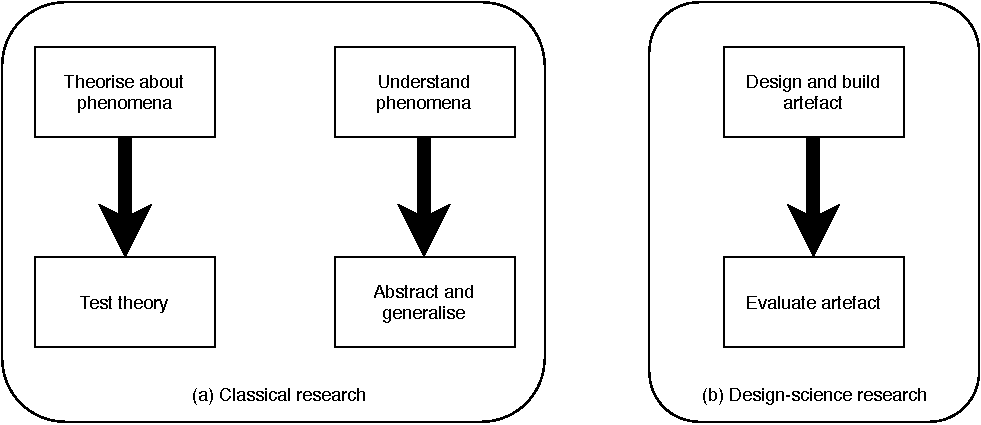
\includegraphics[width=0.9\columnwidth]{TypesOfResearch.pdf}
\begin{figure}[!htb]
    \caption{Risk Profile Setup}
    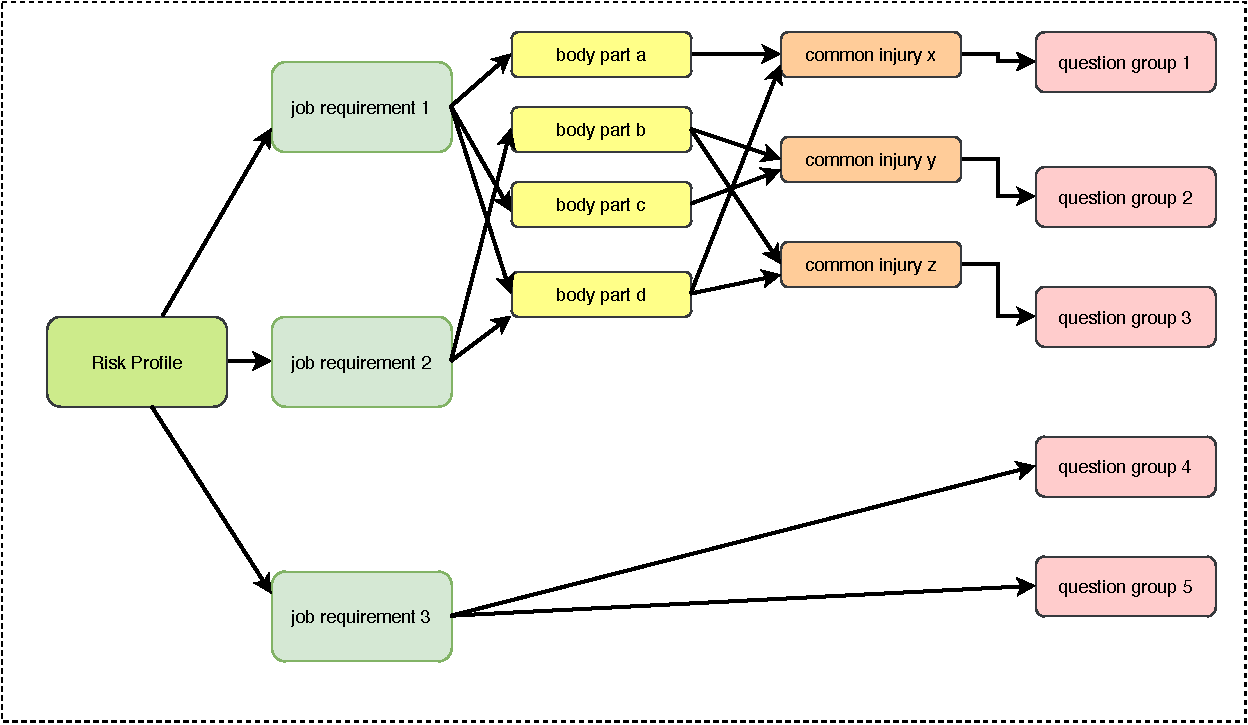
\includegraphics[width=1\columnwidth]{fig/RiskProfile.pdf}
    \label{fig:riskprofile}
\end{figure}



Amongst the outcomes of this research will be the development of a number of novel algorithms to be incorporated into a commercial software product. It is the algorithms that are developed during the design phase that will satisfy the artefact requirement of DSR. The stakeholder community will initially involve the industry partner of the university but will ultimately be useful to anyone dealing with the problem of classifying the answers to closed survey/questionnaire data.



